\section{Evaluation process}
To see how the system complies with the specified solution criteria and how the system can alleviate the problem statement, we carry out an evaluation process. More specifically, we want to evaluate the following:
% What do we look at to evaluate?
\begin{itemize}
\item How close does the regression models reflect reality?
\item Does the routes found based on the weight function reflect reality?
\item Will routes found based on the weight function be faster than original route?
\end{itemize}
% How do we evaluate?
To investigate the above questions, we take the following approach:
\begin{enumerate}
\item First, we select a route $R_{uninformed}=(n_1,...n_m)$ from the GPS data that originates in $n_1$ and ends in $n_m$. We then, directly from the data, determine how long it took to drive this particular route.
\item Secondly, we compute a new weight, $weight(s, t, w)$ for every segment $s=(n_i,n_{i+1}) for 1 \leq i \leq m$ with the weight function described in Section \ref{sec:weight-function}. Let this route, $R_{adjusted}$, be the same route as $R_{uninformed}$ but with the adjusted weights.
\item Here, we compare $R_{uninformed}$ and $R_{adjusted}$ to see if there are any significant changes in the total weight of this route.
\item Now, we traverse the graph to find a new route, $R_{informed}$ originating in $n_1$ and ends in $n_m$ such that the route is the shortest path from $n_1$ to $n_m$ by using the weight of each segment determined by our weight function.
\item We compare $R_{uninformed}$ and $R_{adjusted}$ to see if there are any significant changes in the total weight of this route, and what the difference in the predicted and actual time is.
\item Finally, we compare $R_{informed}$ with $R_{adjusted}$ and see if $R_{informed}$ has chosen a route, that saves time in going from $n_1$ to $n_m$.
\end{enumerate}
The process is illustrated in the graphs in Figure \todo{proc}. Blue nodes represent start nodes, green nodes represent goal nodes where the number in goal nodes are the aggregate weight of all the edges in the route. 

Red arrows represents the uninformed route, where the uninformed route has a weight of 7. The uninformed route with adjusted weights, has a weight of 8. This means that the regression models for the segments has a model accuracy of $\frac{7}{8}=0.875=87.5\%$. 

By computing the informed route based on the regression model weights, the route marked with yellow arrows are found. This informed route has a lower weight than the uninformed route, which means that there can be saved time by 1. T

\begin{figure}
\centering
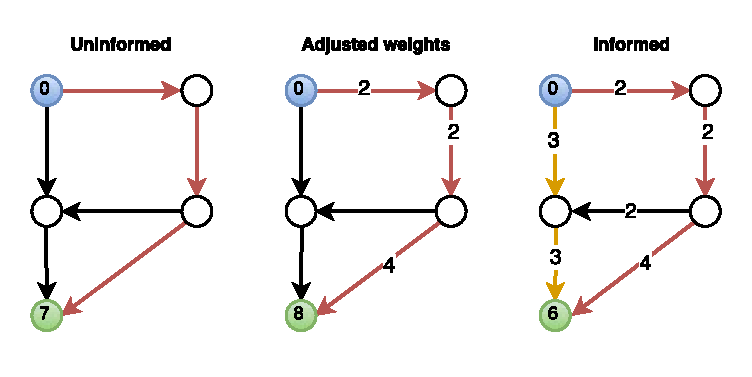
\includegraphics[width=\textwidth]{figures/eval.pdf}
\caption{The evaluation process}
\label{fig:eval}
\end{figure}

We follow the approach on a set of 10 fairly small routes that has no signs of intermedia stops, since intermediate stops in the route, without further measuers taken, would skewer the travel time in favor of our system. 
\begin{table}[]
\centering
\begin{tabular}{llllll}
\textbf{Route} & \textbf{$W_o(R)$} & \textbf{$W_a(R)$}  & \textbf{$W_a(R')$} & \textbf{Model accuracy (\%)} & \textbf{Time saved (\%)} \\ \hline
$r_1$          & 1767              & 2572               & 1726               & 68.7                         & 32.9 \\
$r_2$          & 7023              & 4183               & 2574               & 59.6                         & 38.5 \\
$r_3$          & 2735              & 1793               & 1425               & 65.6                         & 20.5 \\
$r_4$          & 873               & 1010               & 855                & 86.4                         & 15.3 \\
$r_5$          & 5144              & 4915               & 2803               & 95.5                         & 43.0 \\
$r_6$          & 476               & 903                & 620                & 52.7                         & 31.3 \\
$r_7$          & 2432              & 2368               & 1770               & 97.3                         & 25.2 \\
$r_8$          & 2227              & 1431               & 1153               & 64.3                         & 19.4 \\
$r_9$          & 2991              & 13565              & 3250               & 22.0                         & 76.0 \\
$r_{10}$       & 1158              & 1153               & 1101               & 99.6                         & 4.51 \\ \hline
mean       	   &                   &                    &                    & 71.17                        & 30.661
\end{tabular}
\caption{Model accuracy = $100 * \frac{min(W_o(R), W_a(R))}{max(W_o(R), W_a(R))}$\\
	     Time saved = $100 * \frac{W_a(R) - W_a(R')}{W_a(R)}$}
\label{tab:eval-results}
\end{table}
Table \ref{tab:eval-results} shows the time in seconds, $W_0(R)$, for the uninformed route $R$,  the adjusted time, $W_a(R)$, for route $R$, and the informed time $W_a(R)$ for the new route, $R'$.

\textbf{Model accuracy} represents the difference between the uninformed weight and the adjusted weight. The closer the model accuracy for a route is to 100, the better the regression models represents the actual traffic.
 
Time saved represents the time saved for route $r_i$ by traveling the informed route instead of the uninformed route. The higher the time saved the better the informed routing is.

The mean values for model accuracy and time saved shows a mean model accuracy of 71.17\%, which means that the regression models generally underestimates the actual traffic. The mean value for time saved shows that for the tested routes, there are on average 30.661\% time savings by using the systems routefinding.